\subsection{Backward Process: From Surface to Volume}
\label{sec:shifts}

After extracting a base mesh, we build a Frosting layer with a variable thickness and containing Gaussians around this mesh. We want this layer to be thicker in areas where more volumetric rendering is necessary near the surface, such as fuzzy material like hair or grass for example. On the contrary, this layer should be very thin near the parts of the scene that corresponds to well-defined flat surfaces, such as wood or plastic for example.

\begin{figure}[t]
  \centering
  % \includesvg[inkscapelatex=false, width = 1\linewidth]{images/ray.svg}
  % \includesvg[inkscapelatex=false, width = 1\linewidth]{images/ray.svg}
  % \includesvg[inkscapelatex=false, width = 1\linewidth]{images/ray_w_mesh.svg}
  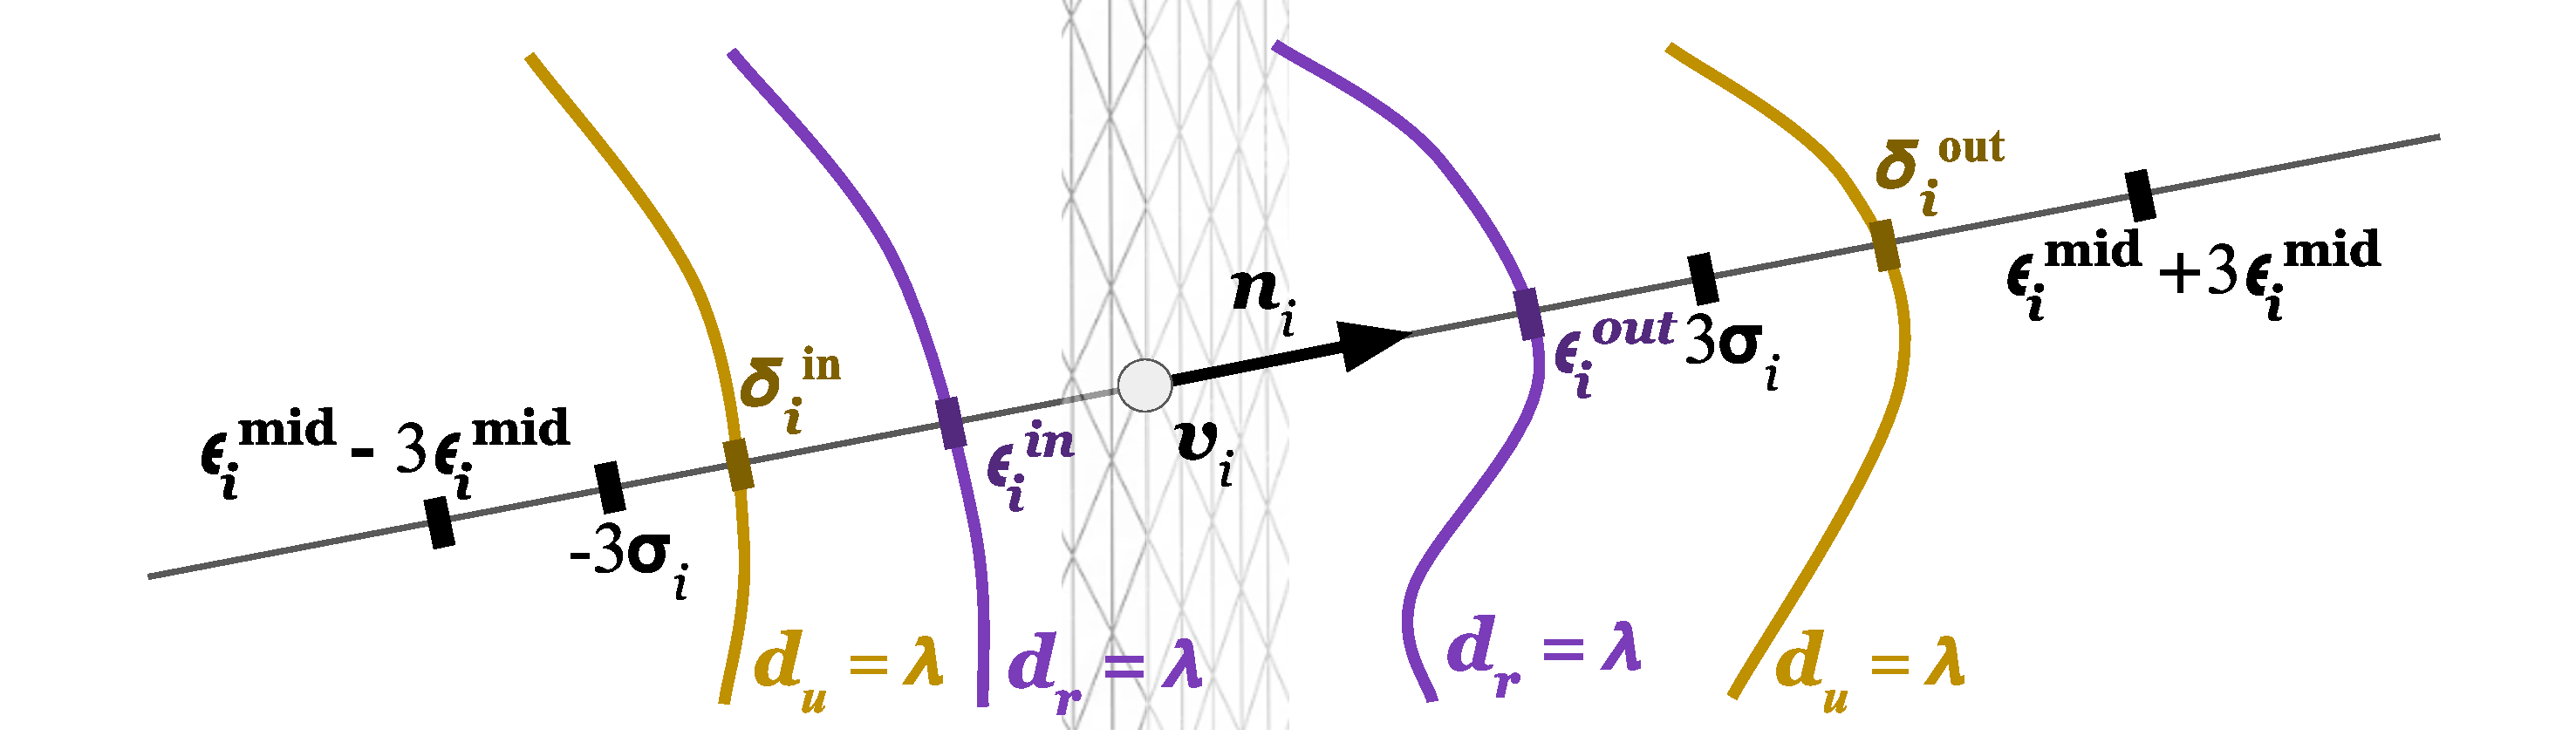
\includegraphics[width=\linewidth]{images/ray_w_mesh.pdf}
  \caption{
  \textbf{How we define the inner and outer bounds of the Frosting layer.} See text in Section~\ref{sec:shifts}.}
  \label{fig:shifts}
\end{figure}


As illustrated in Figure~\ref{fig:shifts}, to define this layer, we introduce two values $\innershift_i$ and $\outershift_i$ for each vertex $\vec{v}_i$ of the extracted base mesh $\calM$. This gives two surfaces with vertices $(\vec{v}_i+\innershift_i \vec{n}_i)_i$ and $(\vec{v}_i+\outershift_i \vec{n}_i)_i$ respectively, where $\vec{n}_i$ is the mesh normal at vertex $\vec{v}_i$. These two surfaces define the inner and outer bounds of the Frosting layer. Note that we do not have to build them explicitly as they directly depend on the base mesh and the $\innershift_i$'s and $\outershift_i$'s.


To find good values for the $\innershift_i$'s and $\outershift_i$'s, we initially tried using directly the unconstrained Gaussians, i.e., the Gaussians obtained before applying the regularization term from SuGaR.  Unfortunately, without regularization, Gaussian Splatting tends to retrieve a thick layer of Gaussians even for ``non-fuzzy'' surfaces, which would result in excessively large values for $\innershift_i$ and $\outershift_i$.  Moreover, the unconstrained Gaussians generally contain many transparent floaters and other outlier Gaussians. Such Gaussians could also bias the shifts toward unnecessarily large values. On the other hand, using only the regularized Gaussians to setup the $\innershift_i$'s and $\outershift_i$'s could miss fuzzy areas since these Gaussians are made flatter by the regularization.


Our solution is thus to consider both the unconstrained and the regularized Gaussians.  More exactly, we estimate the Frosting thickness from the thickness of the unconstrained Gaussians by looking for their isosurfaces, BUT, to make sure we consider the isosurfaces close to the scene surface, we search for the isosurfaces close to the regularized Gaussians: Even under the influence of the regularization term from SuGaR, Gaussians do not align well with the geometry around surfaces with fuzzy details.  As a consequence, the local thickness of the regularized Gaussians is a cue on how fuzzy the material is.


Figure~\ref{fig:shifts}  illustrates what we do to fix the $\innershift_i$'s and $\outershift_i$'s. To restrict the search, we define a first interval $I_i = [-3\sigma_i, 3\sigma_i]$ for each vertex $\vec{v}_i$, where $\sigma_i$ is the standard deviation in the direction of $\vec{n}_i$ of the regularized Gaussian the closest to $\vec{v}_i$. $I_i$ is the confidence interval for the 99.7 confidence level of the 1D Gaussian function of $t$ along the normal. Fuzzy parts result in general in large $I_i$. We could use the $I_i$'s to restrict the search for the isosurfaces of the unconstrained Gaussians. A more reliable search interval $J_i$ is obtained by looking for the isosurfaces of the regularized Gaussians along  $\vec{n}_i$ within $I_i$:
%
\begin{equation}
    \propinnershift_i = \inf ( T ) \text{ , }
    \propoutershift_i = \sup ( T ) \text{ , with }
    T = \left\{ t\in I_i \>\> | \>\> d_r(\vec{v}_i+t\vec{n}_i) \geq \lambda \right\} \> ,
    \label{eq:proposal-shifts}
\end{equation}
%
where $d_r$ is the density function as defined in Eq.~\eqref{eq:gaussian_splatting_density} for the regularized Gaussians.  In practice, we use an isosurface level~$\lambda = 0.01$, i.e., close to zero.
%
We use $ \propinnershift_i$ and $\propoutershift_i$ to define interval $J_i$: $J_i = \left[ \epsilon^\Mid_i - k\epsilon^\half_i, \epsilon^\Mid_i + k\epsilon^\half_i \right]$, with $\epsilon^\Mid_i = (\propinnershift + \propoutershift)/2$ and $\epsilon^\half_i = (\propoutershift - \propinnershift)/2$. We take $k=3$ as it gives an interval large enough to include most of the unconstrained Gaussians while rejecting the outlier Gaussians. Finally, we can compute the inner and outer shifts~$\innershift_i$ and $\outershift_i$ as:
%
\begin{equation}
    \innershift_i = \inf ( V ) \text{ , }
    \outershift_i = \sup ( V ) \text{ , with }
    V = \left\{ t\in J_i \>\> | \>\> d_u(\vec{v}_i+t\vec{n}_i) \geq \lambda \right\} \> .
    \label{eq:shifts}
\end{equation}

\begin{figure}[tb]
  \centering
  \begin{subfigure}{0.155\linewidth}
  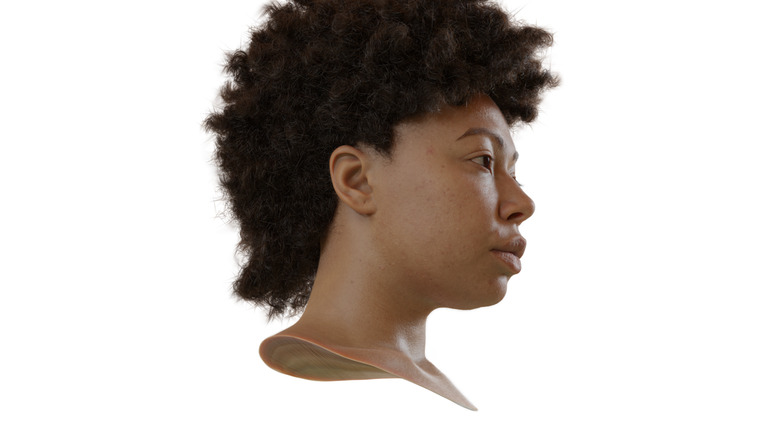
\includegraphics[width=\linewidth]{images/renders/khady_rgb_31.jpg}
  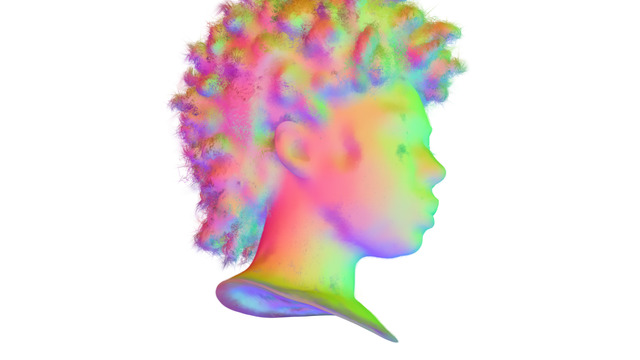
\includegraphics[width=\linewidth]{images/normals/khady_normals_31.jpg}
  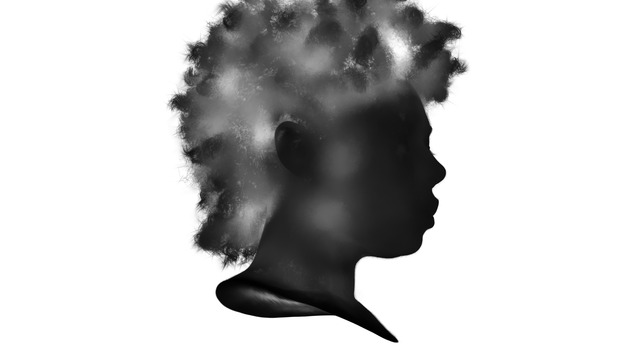
\includegraphics[width=\linewidth]{images/frosting_size/khady_size_31.jpg}
  \end{subfigure}
  %
  \hfill
  %
  \begin{subfigure}{0.155\linewidth}
  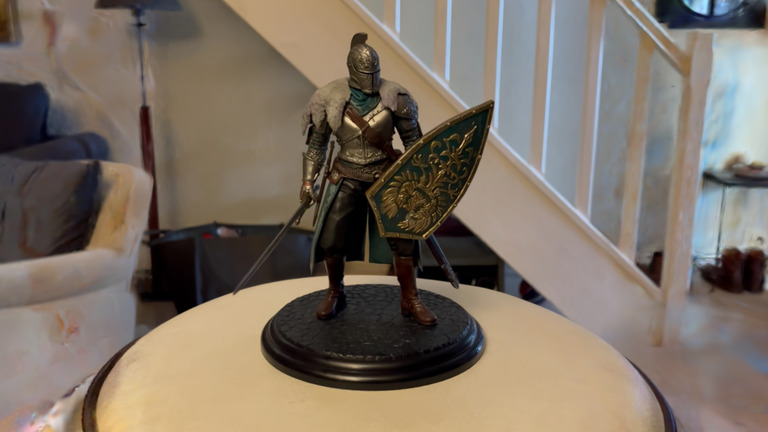
\includegraphics[width=\linewidth]{images/renders/faraam0_rgb_14.jpg}
  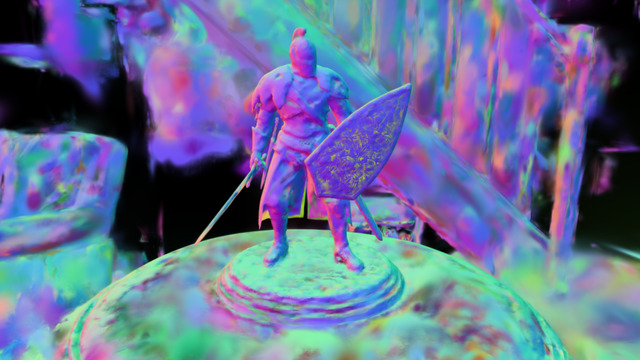
\includegraphics[width=\linewidth]{images/normals/faraam0_normals_14.jpg}
  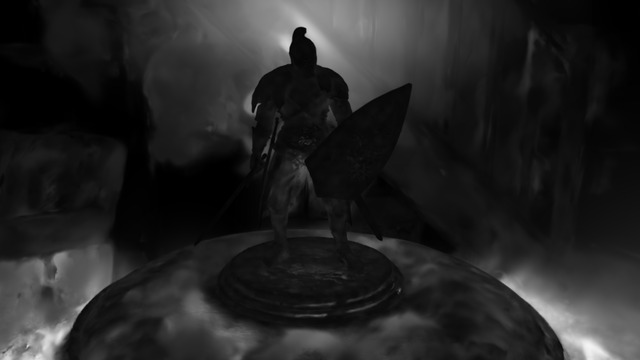
\includegraphics[width=\linewidth]{images/frosting_size/faraam0_size_14.jpg}
  \end{subfigure}
  %
  \hfill
  %
  \begin{subfigure}{0.155\linewidth}
  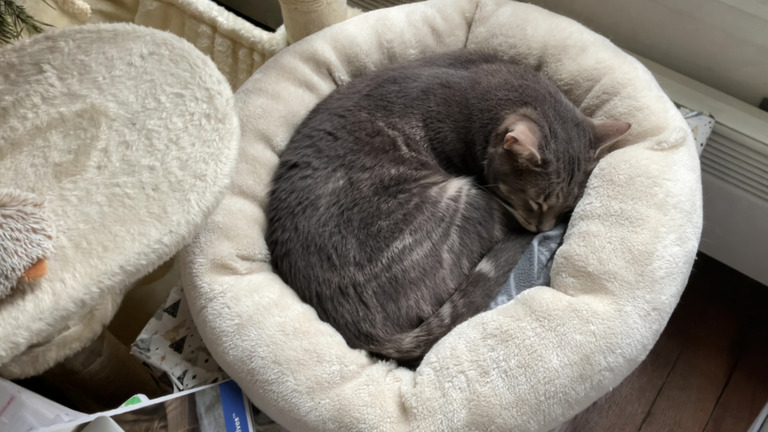
\includegraphics[width=\linewidth]{images/renders/sirius1_rgb_52bis.jpg}
  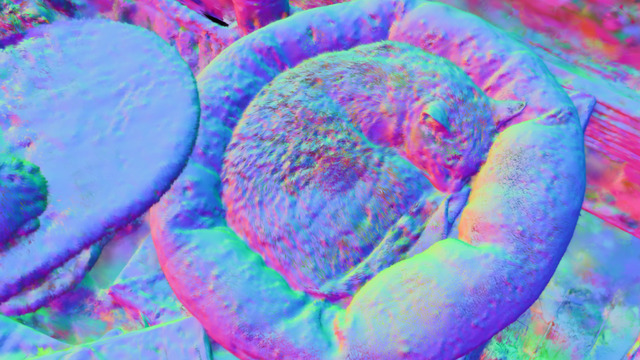
\includegraphics[width=\linewidth]{images/normals/sirius1_normals_52_bis.jpg}
  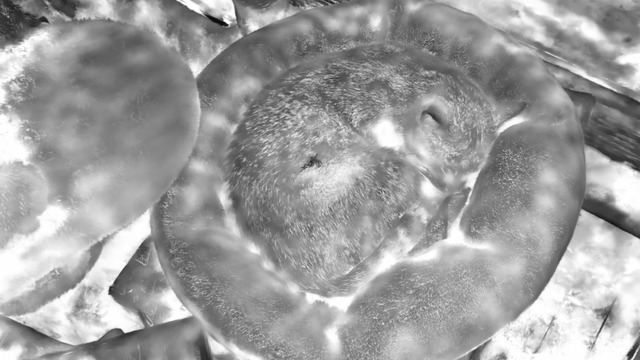
\includegraphics[width=\linewidth]{images/frosting_size/sirius1_size_52_ter.jpg}
  \end{subfigure}
  %
  \hfill
  %
  \begin{subfigure}{0.155\linewidth}
  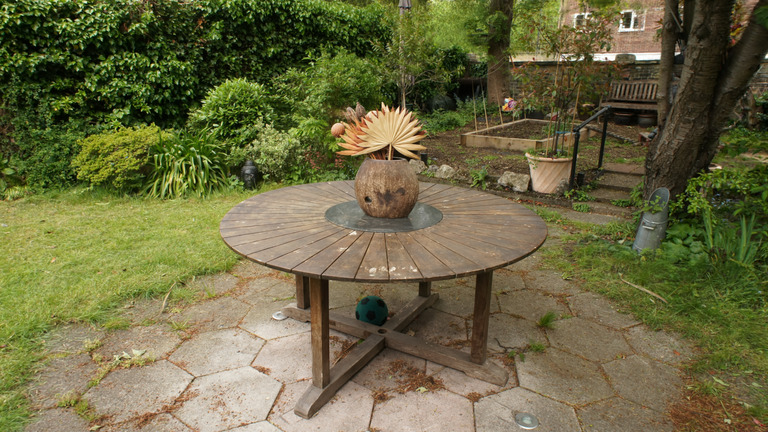
\includegraphics[width=\linewidth]{images/renders/garden_rgb_31.jpg}
  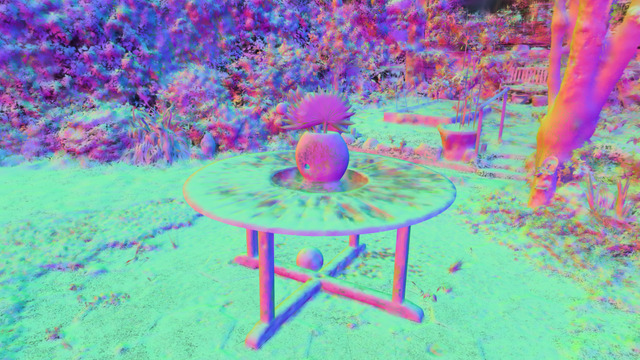
\includegraphics[width=\linewidth]{images/normals/garden_normals_31bis.jpg}
  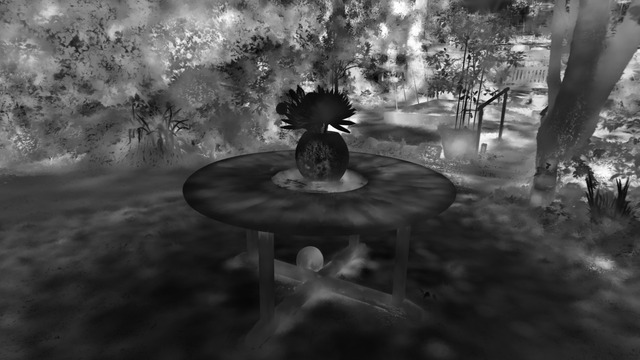
\includegraphics[width=\linewidth]{images/frosting_size/garden_size_31bis.jpg}
  \end{subfigure}
  %
  \hfill
  %
  \begin{subfigure}{0.155\linewidth}
  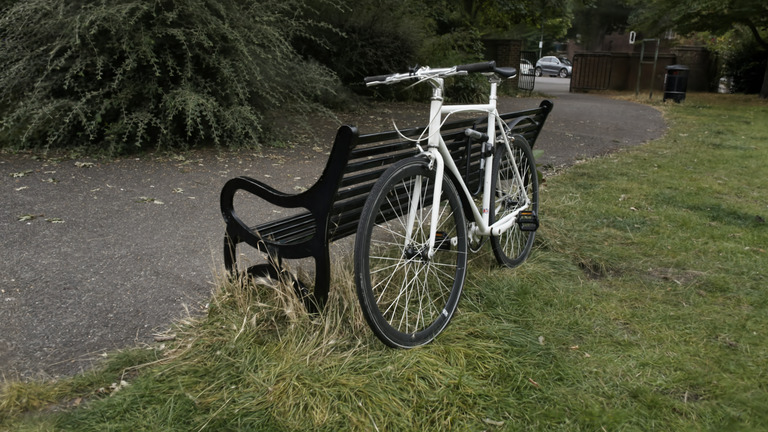
\includegraphics[width=\linewidth]{images/renders/bicycle_rgb_52.jpg}
  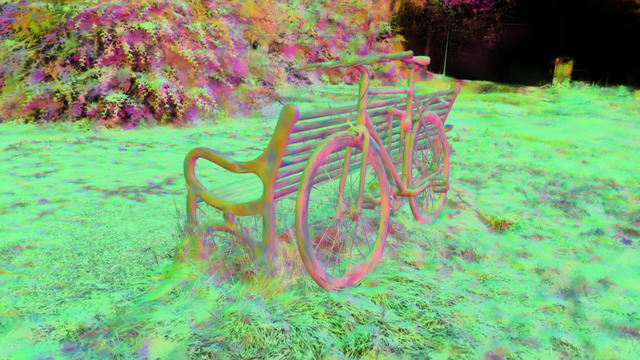
\includegraphics[width=\linewidth]{images/normals/bicycle_normals_52bis.jpg}
  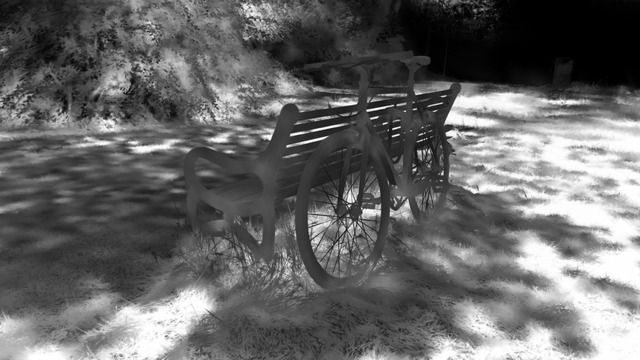
\includegraphics[width=\linewidth]{images/frosting_size/bicycle_size_52bis.jpg}
  \end{subfigure}
  %
  \caption{
  \textbf{Rendering complex scenes with Frosting.} First row: Renderings, Second row: recovered normal maps, Third row: estimated Frosting thickness. Note that the Frosting is thick on fuzzy materials such as the hair and the grass, as expected, and very thin on flat surfaces such as the table on the fourth column.
  }
  \label{fig:frosting-renders}
\end{figure}
